\chapter{Approach and Methodology}\label{approach-and-methodology}

§2 set out the six criteria an automated assessor has to meet. This chapter describes the system built around them and the design used to test it. The first four sections cover the architecture, taking the three agents and the loop they run, then the search pipeline that feeds them evidence, then the deterministic route that computes the nine catalogue questions from harvested portal metadata. The next three cover the evaluation design. They establish the ODMI answer key as the comparator and set out where it is weak, define the eight sampled countries for the final run, and define the measures each result is reported under. The last two sections deal with the controls placed on data leakage and the method behind the experiments.

\section{System Architecture}\label{system-architecture}

The architecture opposes a Researcher agent with an Adversarial Verifier whose job is to disprove, so claims are scrutinised alongside their evidence before they are committed. This adversarial pressure addresses the guessing bias that corroborative checks are vulnerable to, as §2.2 laid out. A second agent asked to confirm findings will tend to ratify a plausible answer, whereas an agent asked to refute aims to produce grounds to do so. A third agent, the Adjudicator, resolves unsettled cases and may decline to answer where neither position prevails.

Requiring the Researcher to return a verbatim passage forms the first half of Attributability, showing exactly where the evidence comes from. The Verifier\textquotesingle s judgement of evidence fit stands in for whether a reasonable reader would agree it entails the claimed answer, so a quote that is real but does not support the label is refused. The Adjudicator\textquotesingle s capacity to abstain is the architecture\textquotesingle s provision for Selectivity, and the thresholds that govern it are set out in §3.2. Every model call writes a record of the model used, the prompt version, the input and output token counts, the latency and the cost, so that any result can be reconstructed from the logged data alone. That record is the traceability half of Reproducibility; the stability half cannot be built in and has to be measured, which §4.6 does. Subgroup Equity and Generalisability are properties of the evaluation rather than of the architecture, and are treated in §4.4 and §4.5 respectively. Nine Quality questions bypass the agents entirely. A deterministic tool computes the figure straight from portal metadata, with no model involved. That gives Convergent Validity a measure that does not rest on the human key, and §3.5 sets out how it works.

\section{The Agent Loop}\label{the-agent-loop}

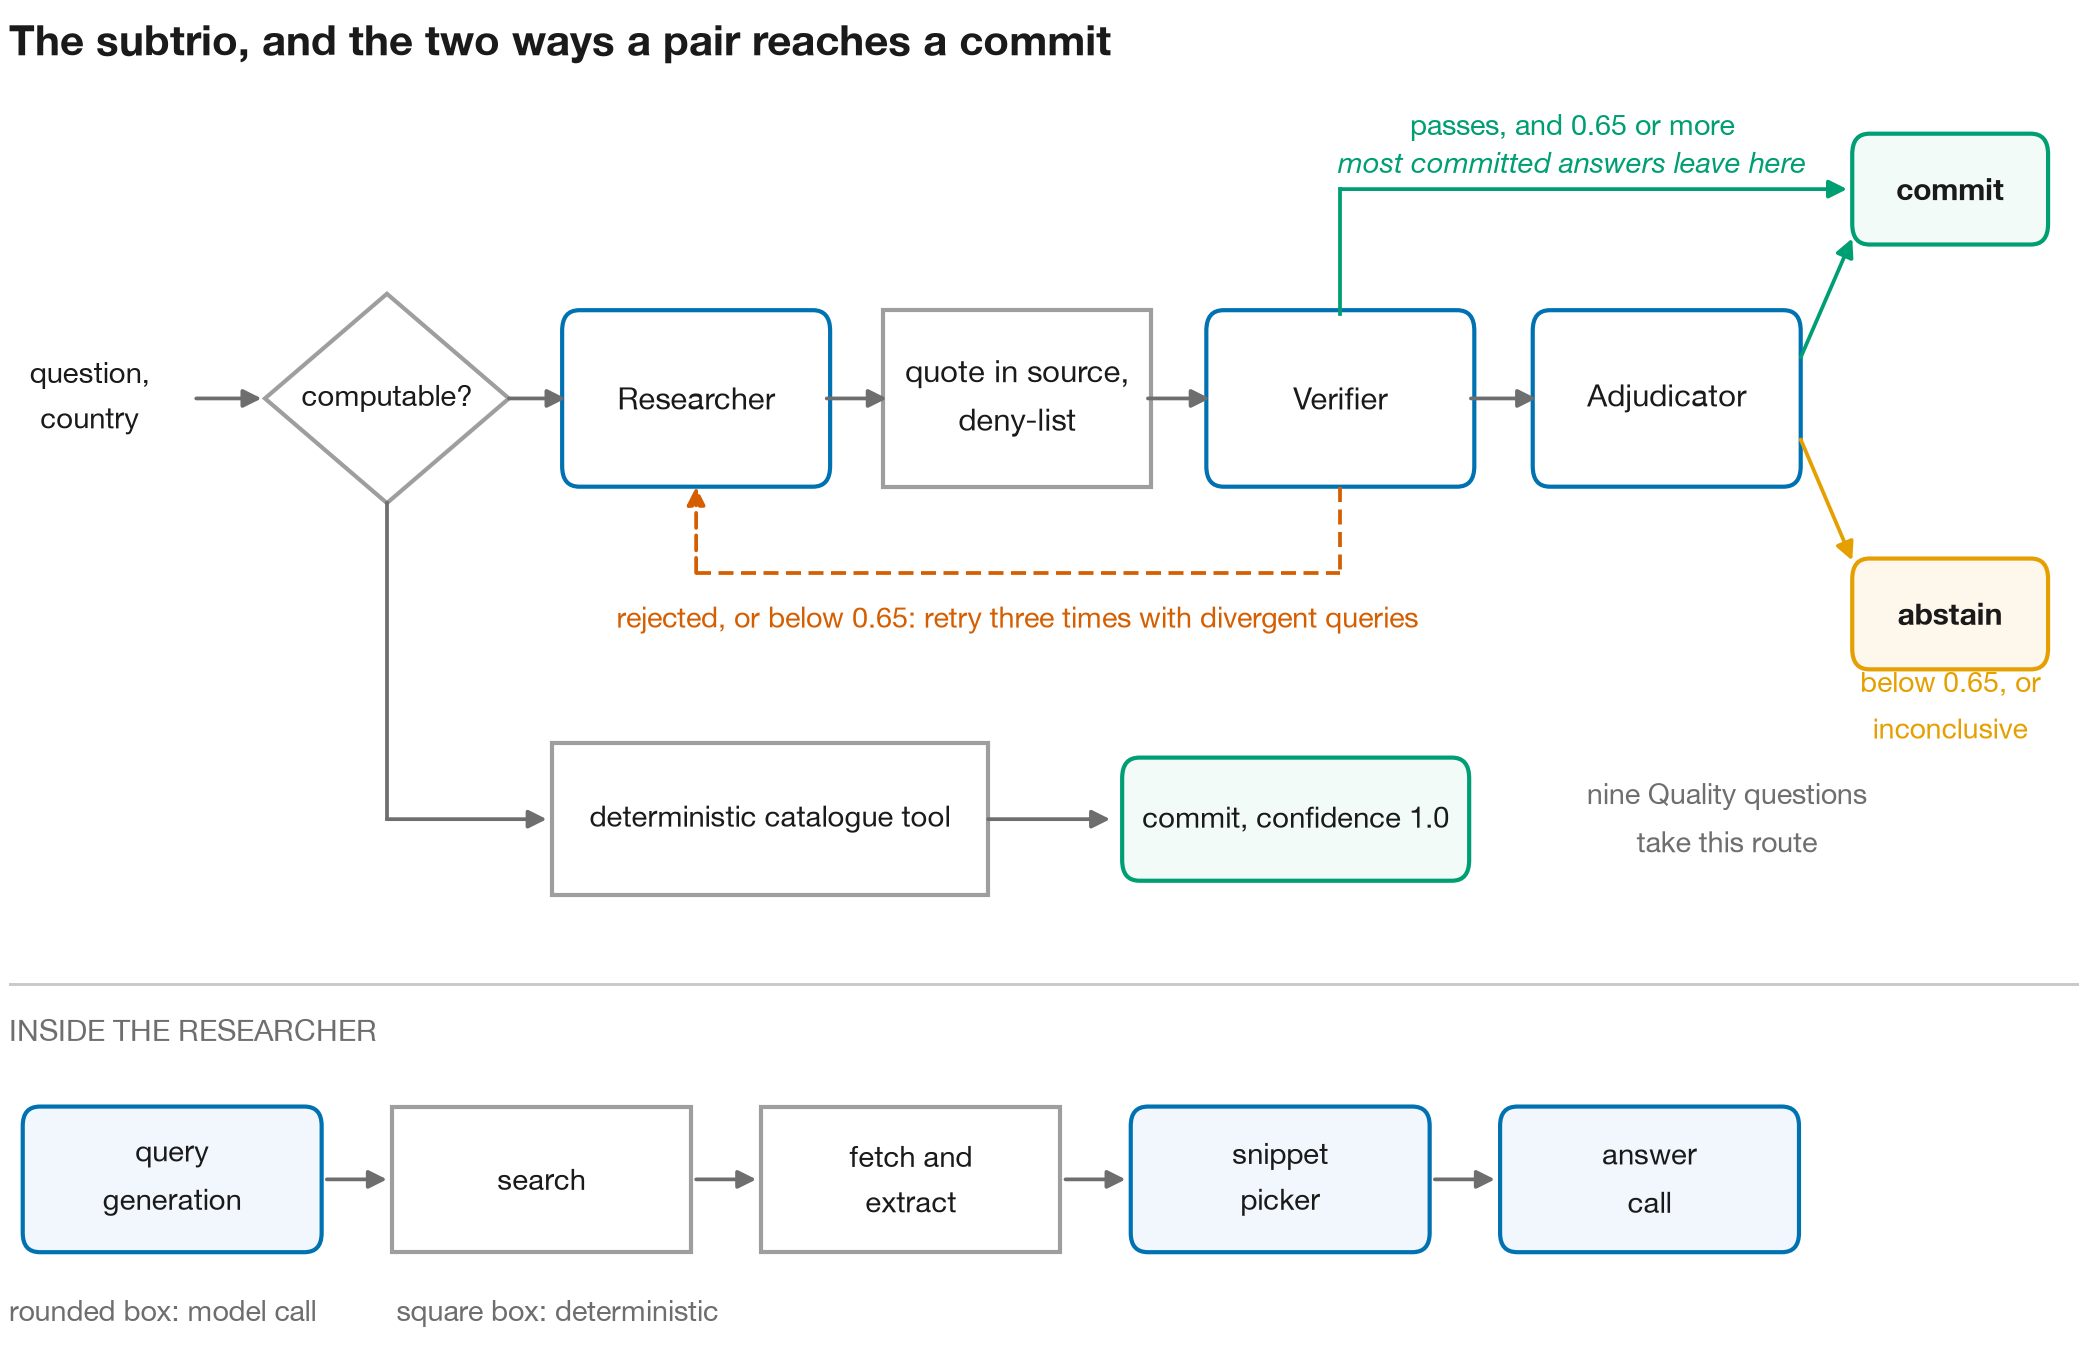
\includegraphics[width=7.08611in,height=4.60208in]{media/media/image6.png}

Figure 3.1: The three agent swarm.

A pair either routes to the deterministic catalogue tool or through the three agents, and reaches a commit by one of two paths.

The Researcher: The first of three model calls converts the question and country into two or three brief search queries, one in English and, if the national language differs, one in that language. The second reads each page the pipeline fetches and keeps the passages relevant to the question, dropping any page that yields none. The third reads the snippets it kept and generates a structured answer comprising a label, a verbatim passage, the source URL, and two confidence scores: one for the evidence found and one for the answer derived from that evidence. The quote and URL make the answer auditable, and the answer confidence is the score the commit threshold acts on.

The Verifier: the verification system comprises several deterministic and probabilistic components. It begins with a deterministic offline gate that checks whether the cited quote appears in the snippet and whether the URL is absent from the deny-list of §3.6. The gate is deliberately lenient in three recorded ways, set out in Appendix B. The system seeks reasons to reject the Researcher\textquotesingle s claim, proceeding through five reasoning steps: substring check, source authority, evidence fit, counterevidence, and verdict. It also conducts an adversarial counter-search for every question, on queries a small model call of its own generates. If the Verifier accepts the answer and the Researcher\textquotesingle s confidence exceeds the final threshold, the pair proceeds to the upper exit shown in Figure 3.1, without an Adjudicator pass. Otherwise, the Verifier returns its counter-argument to the Researcher for a retry.

Commit: If the Verifier passes the answer and the Researcher confidence clears the final floor, the pair commits there, with no Adjudicator pass. Most committed answers leave the loop at this point.

Retry: a rejected or sub-floor answer returns to the Researcher with the Verifier\textquotesingle s counterevidence attached, and the next attempt is forced to diverge from the queries already tried. Without that constraint the retry re-reads the pages that produced the rejected answer, so the loop repeats itself rather than reaching new evidence. Each round therefore enlarges the evidence pool rather than re-arguing over a fixed one. That is the progressive retrieval §2.5 identified as carrying most of Chowdhury et al.\textquotesingle s improvement. Three retries are allowed, so four attempts in all.

The Adjudicator: Only once the retry loop is exhausted, the Adjudicator agent is deployed. It runs no new web searches, and weighs up all the collected evidence throughout the retries from both previous agents. It outputs an authoritative verdict on whether the Researcher, the Verifier or neither was correct, or that the case cannot be settled at all, together with an answer, a confidence, a reasoning string, and the source URL and quote it commits to. If the Adjudicator confidence is below the threshold the answer is not committed.

Confidence threshold: A single threshold governs commitment, 0.65. A Verifier finalises an answer only if the label is not an abstention and the Researcher\textquotesingle s confidence reaches 0.65; otherwise, the pair returns to the retry loop. The same threshold is applied after adjudication, where an Adjudicator answer below 0.65 is rewritten as inconclusive. As detailed in §2.6, the choice of threshold is a policy decision, between balancing accuracy and coverage.

\section{Retrieval}\label{retrieval}

The success of the Researcher depends entirely on the quality of information it can reason over, and as such the search pipeline requires as much thought as the swarm architecture. When the Researcher receives the question-country pair, an LLM call generates three likely search queries that may surface the answer, one in English, an optional native-language query, and an optional query aimed at the national portal. The native-language query exists to surface sources an English query would miss.

The pipeline then runs in stages. Each query is issued to a Google Serper search returning five results. Each result is fetched over httpx, with a Playwright fallback for pages that time out, return an error, or render their content through JavaScript or a web-application firewall. The fetched page is reduced to its main text with the trafilatura Python library, and this extracted text, capped at 16,000 characters, is passed to a Claude snippet picker. The picker scores the candidate passages and returns them ranked best-first. Where one passage clearly dominates it returns that alone; otherwise it returns up to three, each held to 500 characters. The passages taken from a page are then joined into a single snippet, so a three-passage pick runs up to 1,500 characters. At answer time every snippet is truncated to 600 characters before entering the Researcher\textquotesingle s prompt, and up to fifteen snippets reach the answer call. Because the picker ranks passages best-first, this cap retains the strongest evidence and drops a lower-scored tail. That tail is relevant enough to be selected but is the likeliest source of the weak quotes an answer wrongly settles on, and the cap also shortens the run. The pipeline caches at three levels, the search result, the page fetch and the picked snippet, each for thirty days, so that repeated runs are reproducible and cheap. 

\section{Ground Truth and Its Limits}\label{ground-truth-and-its-limits}

The swarm\textquotesingle s accuracy is marked against the 2025 ODMI assessment answers, as it is the closest publicly available ground truth. It provides all 5,148 answers across every question-country pair, each one self-reported by the country and then reviewed by Capgemini, who confirm 63\% of answers, supplement 27\% of answers with more evidence, and actively change around 10\%. The evidence attached to an answer ranges from a clear URL to a more informal comment from a national data team such as \textquotesingle We are working on it\textquotesingle. In §4, the term `gold' refers to the answer in the ground truth set, for example `negative-golds' means the questions in the 2025 questionnaire that were answered with a ``no'' or low band. Table 3.1 shows the breakdown of question type, with the majority requiring a binary answer.

{\def\LTcaptype{none} % do not increment counter
\begin{longtable}[]{@{}
  >{\raggedright\arraybackslash}p{(\linewidth - 4\tabcolsep) * \real{0.5000}}
  >{\centering\arraybackslash}p{(\linewidth - 4\tabcolsep) * \real{0.2500}}
  >{\centering\arraybackslash}p{(\linewidth - 4\tabcolsep) * \real{0.2500}}@{}}
\toprule\noalign{}
\begin{minipage}[b]{\linewidth}\raggedright
\textbf{Answer shape}
\end{minipage} & \begin{minipage}[b]{\linewidth}\centering
\textbf{Count}
\end{minipage} & \begin{minipage}[b]{\linewidth}\centering
\textbf{Share}
\end{minipage} \\
\midrule\noalign{}
\endhead
\bottomrule\noalign{}
\endlastfoot
Binary (yes / no) & 124 & 87\% \\
Percentage-band & 12 & 8\% \\
Ordinal-magnitude & 3 & 2\% \\
Count-band & 2 & 1\% \\
Categorical & 2 & 1\% \\
\textbf{Total} & \textbf{143} & \textbf{100\%} \\
\end{longtable}
}

Table 3.1: Answer shapes across the 143 questions.

Rating accuracy as the match rate with this ground-truth is not perfect. The answers originate with the country, and 29 of the questions ask about internal practice where evidence is hard to find online, such as \textquotesingle Do you monitor search keywords?\textquotesingle{} or \textquotesingle Do you monitor portal traffic?\textquotesingle (Appendix D lists all 29). Across all 36 countries these 29 questions are answered ``yes'' 79.3\% of the time, which confounds whether the system is successfully retrieving the relevant information and reasoning carefully over it, or whether the architecture has not addressed the natural LLM optimism bias and both Researcher and Verifier have been misled by vague or missing evidence. This points to a class of error that sits outside the declared ground-truth mismatches, and isolating it is an necessary step towards true reliability. Secondly, many of the calculated answers for the nine deterministic questions diverge from the reported figures, as shown in §3.5, so the ground truth is demonstrably wrong on at least some items. 

These two flaws change how the evaluation has to be framed. Where the swarm and the ODMI disagree, it can be unclear whether the swarm is wrong or the ODMI is, and Fumega and Gao (2026) found that an agentic assessor is sometimes right where the human experts are not. Neither rater is infallible here, since the swarm can misread evidence and the human key is self-reported and diverges from the recompute. §4.1 takes this up again, doing an independent audit of 94 false positives across eight countries, to see where the system falls short, and which questions are structurally out-of-reach for a closed-world assessment.

\section{Deterministic Tool for Catalogue Questions}\label{deterministic-tool-for-catalogue-questions}

Nine Quality questions ask for a proportion of the national catalogue, for example the share of datasets conforming to DCAT-AP, which is directly computable. The only pooled public source for the same figures is the Metadata Quality Assessment (MQA) on data.europa.eu, which is deny-listed because that domain also publishes the assessment\textquotesingle s own answers. A deterministic tool computes them instead, with no language model involved at any stage.

Each catalogue question asks a national team to select a percentage band for its own portal, that band carries a score, and Capgemini confirms or amends what the team submits. Across the thirty-six countries the key records 280 confirmations against 44 amendments, so in every case there was a submitted answer for a reviewer to rule on. The self-report shows plainly wherever a team was challenged, with countries defending their own portal in the first person, several replying directly to a reviewer\textquotesingle s remark, and one answering ``i don\textquotesingle t know''. Two national teams cite the MQA as the basis of their numbers. What sits behind the rest is thinner. Of the 324 rows, 87 leave the evidence box empty and a further 207 carry only the string `N/A', so nine in ten offer nothing to check, and 86\% were confirmed with no amendment. On this group the assessment accepts a self-reported figure with nothing attached to support it.

The tool can only harvest a country whose portal route is known, so classification comes first. A stack-fingerprinting prober covering CKAN, uData, paged DCAT-AP, SPARQL, piveau, OpenDataSoft and data.json portals identifies each national portal and records the route in a registry, verified against a one-page sample before the route is trusted. 22 of the 36 countries carry a registry entry. The harvester then pages the catalogue and stores the retrieved metadata as a snapshot with a SHA-256 of its contents, and the nine metric functions run over that stored snapshot. Conformance is scored against the SEMIC DCAT-AP SHACL. Nine countries hold at least one complete snapshot, and several harvests failed part way and are flagged as partial, most often on a read timeout or a DNS error. The recompute in Table 3.2 exposes gaps in the self-reported figures, running in both directions. France reports over 90\% licence coverage against a recomputed 37.8\% over a sample of five thousand datasets. Romania reports 10-30\% on recommended DCAT-AP property usage and under 10\% on optional usage, against a recompute of 100\% and 99.7\%.

Table 3.2: Full and sampled harvests of national data portals, showing agreement across the nine computable Quality questions.

{\def\LTcaptype{none} % do not increment counter
\begin{longtable}[]{@{}
  >{\raggedright\arraybackslash}p{(\linewidth - 22\tabcolsep) * \real{0.0282}}
  >{\raggedright\arraybackslash}p{(\linewidth - 22\tabcolsep) * \real{0.0993}}
  >{\centering\arraybackslash}p{(\linewidth - 22\tabcolsep) * \real{0.0484}}
  >{\centering\arraybackslash}p{(\linewidth - 22\tabcolsep) * \real{0.0418}}
  >{\centering\arraybackslash}p{(\linewidth - 22\tabcolsep) * \real{0.0338}}
  >{\centering\arraybackslash}p{(\linewidth - 22\tabcolsep) * \real{0.0538}}
  >{\centering\arraybackslash}p{(\linewidth - 22\tabcolsep) * \real{0.0538}}
  >{\centering\arraybackslash}p{(\linewidth - 22\tabcolsep) * \real{0.0538}}
  >{\centering\arraybackslash}p{(\linewidth - 22\tabcolsep) * \real{0.0538}}
  >{\centering\arraybackslash}p{(\linewidth - 22\tabcolsep) * \real{0.0418}}
  >{\centering\arraybackslash}p{(\linewidth - 22\tabcolsep) * \real{0.0418}}
  >{\centering\arraybackslash}p{(\linewidth - 22\tabcolsep) * \real{0.0553}}@{}}
\toprule\noalign{}
\begin{minipage}[b]{\linewidth}\centering
\end{minipage} & \begin{minipage}[b]{\linewidth}\centering
\textbf{Source}
\end{minipage} & \begin{minipage}[b]{\linewidth}\centering
\textbf{n}
\end{minipage} & \begin{minipage}[b]{\linewidth}\centering
\textbf{Q12}
\end{minipage} & \begin{minipage}[b]{\linewidth}\centering
\textbf{Q13}
\end{minipage} & \begin{minipage}[b]{\linewidth}\centering
\textbf{Q16}
\end{minipage} & \begin{minipage}[b]{\linewidth}\centering
\textbf{Q17}
\end{minipage} & \begin{minipage}[b]{\linewidth}\centering
\textbf{Q18}
\end{minipage} & \begin{minipage}[b]{\linewidth}\centering
\textbf{Q21}
\end{minipage} & \begin{minipage}[b]{\linewidth}\centering
\textbf{Q22}
\end{minipage} & \begin{minipage}[b]{\linewidth}\centering
\textbf{Q25}
\end{minipage} & \begin{minipage}[b]{\linewidth}\centering
\textbf{Q27}
\end{minipage} \\
\midrule\noalign{}
\endhead
\bottomrule\noalign{}
\endlastfoot
\textbf{AL} & \emph{Self-reported} & & \emph{\textgreater90\%} & \emph{5-10} & \emph{\textgreater90\%} & \emph{\textgreater90\%} & \emph{\textgreater90\%} & \emph{\textgreater90\%} & \emph{\textgreater90\%} & \emph{\textgreater90\%} & \emph{\textgreater90\%} \\
& DCAT-AP API & 130 & \textbf{100.0} & -\/- & -\/- & -\/- & -\/- & \textbf{100.0} & -\/- & \textbf{100.0} & -\/- \\
\textbf{DE} & \emph{Self-reported} & & \emph{\textgreater90\%} & \emph{5-10} & \emph{\textgreater90\%} & \emph{\textgreater90\%} & \emph{71-90\%} & \emph{31-50\%} & \emph{\textgreater90\%} & \emph{\textgreater90\%} & \emph{71-90\%} \\
& DCAT-AP RDF & 3,000 & \textbf{100.0} & 13 & 4.2 & \textbf{100.0} & 100.0 & 2.7 & \textbf{100.0} & \textbf{99.9} & 45.6 \\
\textbf{FR} & \emph{Self-reported} & & \emph{\textgreater90\%} & \emph{1-4} & \emph{\textgreater90\%} & \emph{\textgreater90\%} & \emph{\textgreater90\%} & \emph{\textgreater90\%} & \emph{\textgreater90\%} & \emph{\textgreater90\%} & \emph{\textgreater90\%} \\
& DCAT-AP RDF & 1,000 & 66.9 & 6 & 69.5 & \textbf{100.0} & \textbf{100.0} & \textbf{100.0} & \textbf{100.0} & 66.6 & 67.6 \\
& DCAT-AP RDF & 5,000 & 37.8 & 7 & 31.9 & \textbf{100.0} & \textbf{100.0} & \textbf{100.0} & \textbf{100.0} & 37.7 & 40.5 \\
\textbf{HU} & \emph{Self-reported} & & \emph{\textgreater90\%} & \emph{1-4} & \emph{\textgreater90\%} & \emph{\textgreater90\%} & \emph{\textgreater90\%} & \emph{\textgreater90\%} & \emph{\textgreater90\%} & \emph{\textless10\%} & \emph{\textgreater90\%} \\
& CKAN & 2,282 & 72.8 & \textbf{2} & \textbf{100.0} & \textbf{100.0} & \textbf{100.0} & \textbf{100.0} & \textbf{100.0} & \textbf{1.9} & \textbf{96.4} \\
\textbf{NL} & \emph{Self-reported} & & \emph{\textgreater90\%} & \emph{5-10} & \emph{\textgreater90\%} & \emph{\textgreater90\%} & \emph{10-30\%} & \emph{51-70\%} & \emph{\textgreater90\%} & \emph{\textgreater90\%} & \emph{\textgreater90\%} \\
& CKAN & 20,772 & \textbf{96.9} & \textbf{7} & 66.6 & \textbf{100.0} & 86.3 & 100.0 & \textbf{100.0} & \textbf{90.3} & 50.6 \\
\textbf{RO} & \emph{Self-reported} & & \emph{\textgreater90\%} & \emph{1-4} & \emph{71-90\%} & \emph{10-30\%} & \emph{\textless10\%} & \emph{\textgreater90\%} & \emph{\textless10\%} & \emph{\textgreater90\%} & \emph{31-50\%} \\
& CKAN & 5,143 & \textbf{96.2} & 5 & 96.1 & 100.0 & 99.7 & \textbf{99.8} & 99.8 & \textbf{96.2} & 62.3 \\
\end{longtable}
}

Recomputed values are percentages, except Q13 which is a count of distinct licences. Bold marks a recompute falling in the band the country reported: 31 of 66 across the eight complete harvests. Partial harvests are excluded. 

\section{Data-Leakage Controls}\label{ccdata-leakage-controlscc}

Scoring against ODMI\textquotesingle s published responses creates a retrieval hazard because these responses sit on data.europa.eu, and any page reproducing them provides the answer the system is meant to derive. A single deny-list, imported by every retrieval path, contains twelve domains and five URL path fragments. The domains cover ODMI\textquotesingle s publishing surface (\emph{data.europa.eu, publications.europa.eu, op.europa.eu, europeandataportal.eu}); the archives that serve a page after the original moves (\emph{web.archive.org, archive.org, archive.today, archive.ph, archive.is}); and the caches that return a copy without reaching the origin (\emph{webcache.googleusercontent.com, cache.google.com, cachedview.com}). Host matching runs on the suffix, so subdomains fall with their parent. The fragments \emph{open-data-maturity, /odmi, 2024\_odm\_questionnaire, 2025\_odm\_questionnaire} and \emph{merged\_respons}es catch ODMI material republished on permitted domains.

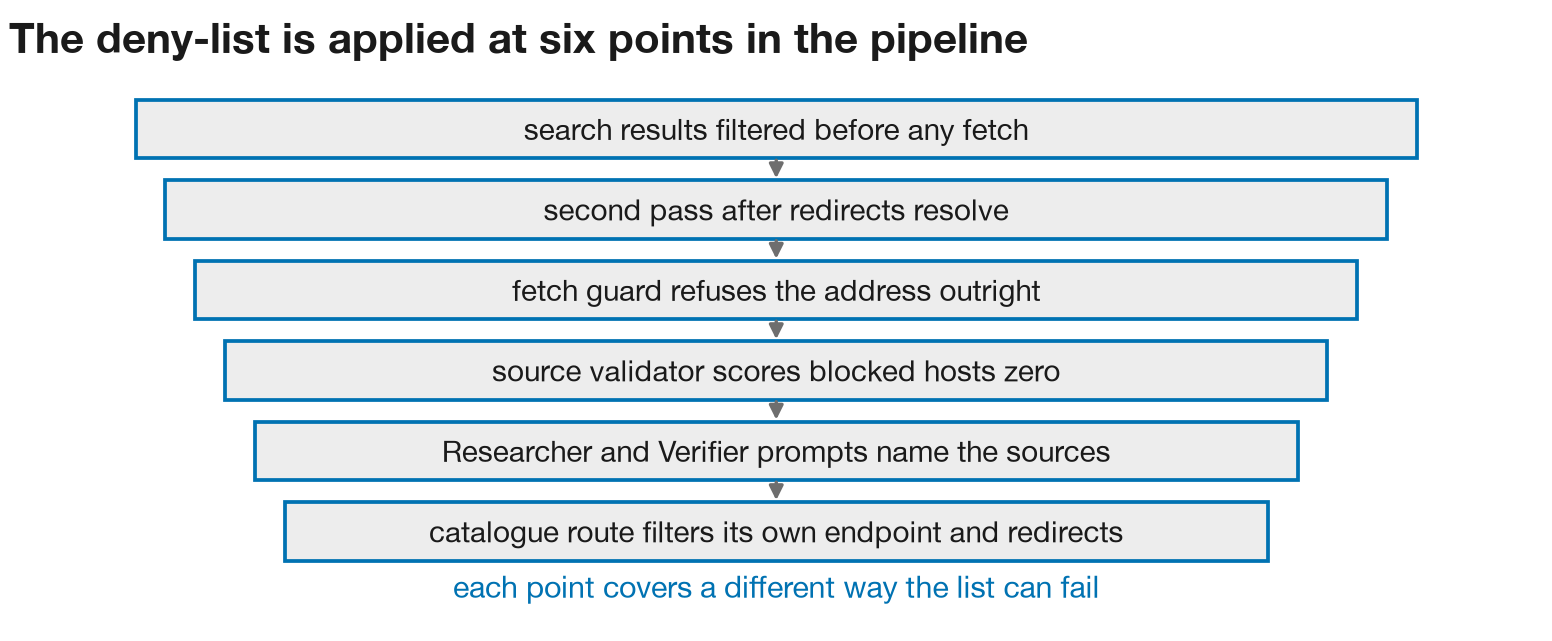
\includegraphics[width=7.08611in,height=2.92222in]{media/media/image7.png}

Figure 3.2: The six points at which the deny-list is applied.

Six points in the pipeline apply the deny-list, and Figure 3.2 sets out how each covers a different way it can fail. The search stage removes blocked results before they are fetched, and a second pass checks the set again afterwards in case a redirect has led somewhere blocked. The fetch guard refuses the address before any request is sent, and records the refusal against that question. The source validator gives blocked domains a trust score of zero, which stops them being used as evidence. The Researcher and Verifier prompts both name the forbidden sources and tell the agents not to use them. The deterministic catalogue route applies the same list to its own endpoint and to every redirect it follows.

Prior knowledge escapes retrieval controls entirely, since a model trained on text containing the published answers could reproduce them without issuing a query. The 2025 ODMI report was published on 19 December 2025, within the January 2026 training-data window of Sonnet 4.6. A closed-book probe bounds it empirically by repeating an evaluation with retrieval disabled, and the resulting accuracy is compared against the score a system would reach by answering ``yes'' to every binary question, 59.4\% on these eight countries. A model reciting a memorised key would beat that baseline; a model without one would not. Republication of the answer key on a permitted domain remains uncontrolled, since a consultancy write-up or news summary can restate a country\textquotesingle s answers without a listed host or fragment, and content-level fingerprinting of the published answers has not been built.

\section{Evaluation Set}\label{evaluation-set}

All tuning ran on a development set of five countries. The Netherlands and Malta served as balanced cases no-share, the proportion of a country\textquotesingle s binary questions whose published answer is ``no'', at 22\% and 31\%, Albania at 23\% with a low-resource language and a small open-data estate, and Norway and France as near-uniform yes cases at 8\% and 1\%. The 156-pair tuning battery ran on Malta, the Netherlands and Albania, picking out all their no golds and an equal number of randomly chosen yes gold questions. The threshold sweeps, the choice of retrieval pipeline, the search scope, the snippet cap and the ablations in §4.7 were all run on this set, leaving the evaluation countries untouched by tuning. The full list of experiments run for both tuning and results is detailed in Appendix C.

A system carrying an unchecked optimism bias scores well simply by answering ``yes'', and it scores best against the countries that answer ``yes'' most. A false-positive rate can only be measured where the key says ``no'', and those answers concentrate in the low-maturity tail, falling from 85\% of Bosnia's binary questions to none of Lithuania's. Discrimination is therefore only observable at the low-maturity end of the range, among countries that also tend not to meet many of the requirements a high-quality portal is scored on. The evaluation set therefore oversamples countries where negative golds are dense, since a random sample would be dominated by all-yes responses and the false-positive rate would rest on too few items to interpret. A further consequence is that countries are less likely to publish evidence that their open data falls short than evidence that it complies, so lower-maturity countries are expected to abstain more often.

Throughout development, eight countries were held out from all tuning to form the evaluation set, chosen on language resource level and overall no-share. Resource level is taken from the six-class taxonomy of Joshi et al. (2020), which grades a language from 0 to 5 on the labelled and unlabelled data available for it. Stratum A takes the four highest no-share countries outside the development set whose main language sits at class 3 or below, which gives Bosnia and Herzegovina, North Macedonia, Montenegro and Bulgaria. Stratum B takes the four highest at class 4 or above, giving Finland, Croatia, Sweden and Belgium. Figure 3.3 places each country at its class. Montenegrin is not listed, but it is a variety of the same South Slavic language as Bosnian, so it is read here as class 3. Between them the eight carry 1,144 question-country pairs and 368 binary negative golds, 261 of which sit in stratum A. The taxonomy predates the current generation of multilingual models and records catalogued resource counts rather than measured comprehension.

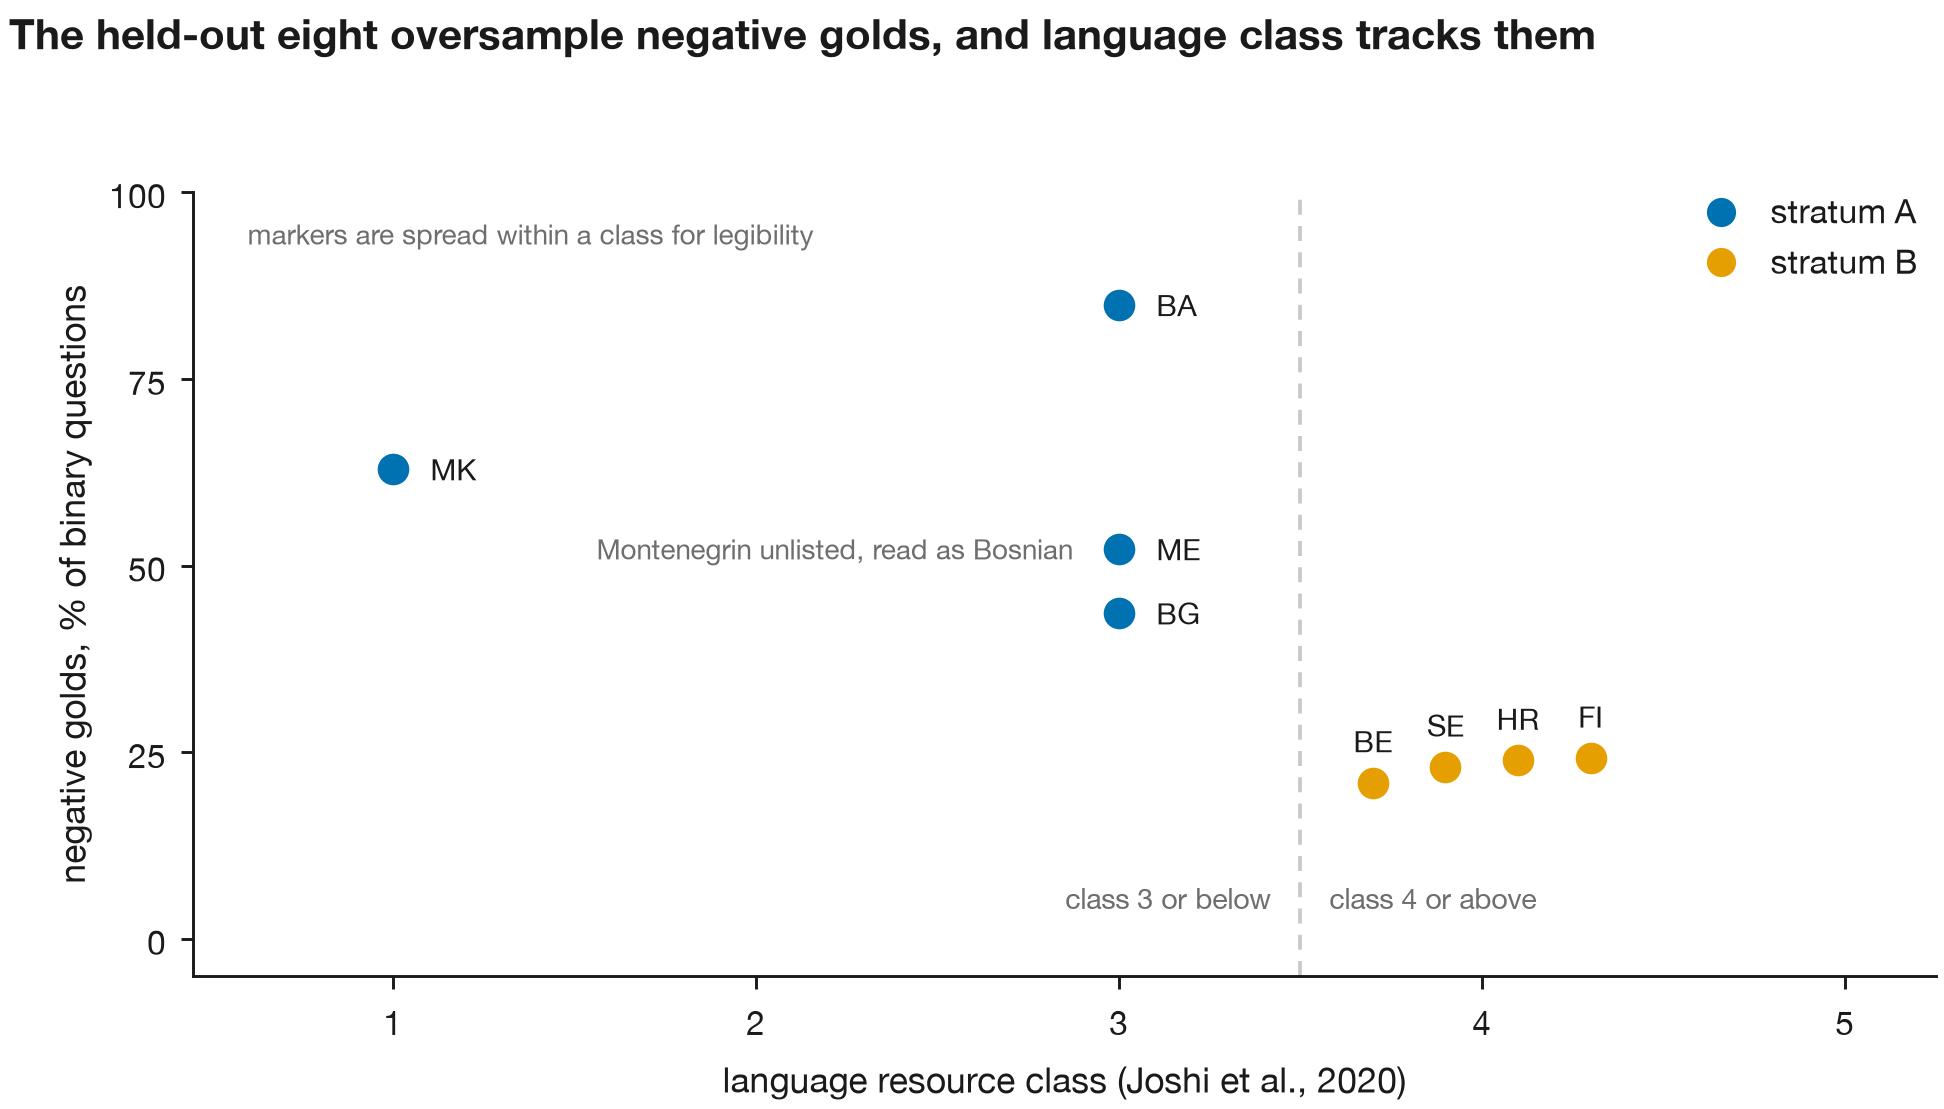
\includegraphics[width=7.08611in,height=4.03889in]{media/media/image8.png}

Figure 3.3: The evaluation eight by language resource class and negative-gold share.

§2.7 outlines three reasons a country might score poorly: the model misreads native-language evidence, the evidence is absent from the web, or the country is less open. The strata address the first reason. A markedly higher false-positive rate in stratum A would show that weaker comprehension of a national language makes the system commit wrong answers rather than making it decline. Conversely, a stable rate across strata indicates that success depends more on evidence retrieval. The strata are not matched for maturity, as Figure 3.3 shows. Stratum A ranges from 43.6\% `no-share' in Bulgaria to 84.8\% in Bosnia, while stratum B spans 20.9\% in Belgium to 24.2\% in Finland. Thus language class and maturity co-vary, and a result in stratum A bounds the language effect instead of isolating it.

\section{Experiments}\label{experiments}

The experimental programme divides into two classes, those used to tune the system in development, and those used to derive the results in §4. The tuning experiments settle design questions inside the system, for example, whether the Verifier issues its own counter-search, how many results each query returns, how broadly each query searches, and which variant of the Researcher prompt is used. All of these run on the development countries, and each is dispatched with an adoption rule written in advance, stating what result would displace the incumbent setting and by what margin. The results experiment is a single run of one frozen configuration of the architecture across the eight evaluation countries, which are not touched during any tuning experiment.

Every experiment is registered before dispatch, in a design note fixing the question, the sample, the endpoint and the adoption rule, and in a machine-readable row recording the same design. The orchestrator refuses to start a run that breaks any of five conditions, listed in Appendix C, and each is a hard failure that halts the run before any expenditure. The two that bear on the results are that no specification may name an evaluation country, and that experiments varying retrieval or measuring cost are forced onto a cold cache, since the search cache is keyed on the query and two arms sharing a warm cache would read one another's evidence. A single declared exception exists for the full results run, which must contain no development country.

Many experiments found no improvement on the incumbent design, particularly on the reasoning side. Where an arm did not clear its rule, the incumbent setting was retained and the null result was recorded in the same way as any other outcome.

The completed experiments are set out in §8.3, together with the question each addresses, its sample, its arms and its adoption rule.

The analysis that produces the figures reported in §4 is itself under test, as are the constraints above, which fail visibly if they are removed.

\section{Metrics}\label{metrics}

The following metrics, set out in Table 3.3, will be used in §4 to evaluate the results.

Table 3.3: Metrics reported in §4.

{\def\LTcaptype{none} % do not increment counter
\begin{longtable}[]{@{}
  >{\raggedright\arraybackslash}p{(\linewidth - 4\tabcolsep) * \real{0.2451}}
  >{\raggedright\arraybackslash}p{(\linewidth - 4\tabcolsep) * \real{0.5196}}
  >{\raggedright\arraybackslash}p{(\linewidth - 4\tabcolsep) * \real{0.2353}}@{}}
\toprule\noalign{}
\begin{minipage}[b]{\linewidth}\raggedright
\textbf{Metric}
\end{minipage} & \begin{minipage}[b]{\linewidth}\raggedright
\textbf{What it measures}
\end{minipage} & \begin{minipage}[b]{\linewidth}\raggedright
\textbf{Denominator}
\end{minipage} \\
\midrule\noalign{}
\endhead
\bottomrule\noalign{}
\endlastfoot
Coverage & Share of attempted pairs the system commits to. The complement of the abstention rate & All attempted pairs \\
Commit-accuracy & Share of committed answers matching the key & Scorable committed pairs \\
Per-class recall & Share of one gold class answered correctly, reported separately for yes and no golds & All golds in the class, and committed golds alone \\
Negative-gold false-positive rate & Share of negative golds the system answered ``yes''. A negative gold is one whose key answer is no, or a low band & All negative golds, and committed negative golds alone \\
Balanced accuracy & Mean of the true-positive and true-negative rates, removing the class imbalance that raw accuracy rewards. 0.5 is the floor, and below it the system is doing worse than answering the same way every time & Binary gold pairs \\
Expected calibration error & Mean gap between stated confidence and observed accuracy, weighted by bin size. Zero is perfect & Committed answers, binned by stated confidence \\
Selective risk & Accuracy against surviving coverage as the commit threshold sweeps upward & Pairs surviving at each threshold \\
McNemar\textquotesingle s test & Whether two systems differ, using only the items on which they disagree. A small p is evidence of a real difference; a high p does not establish equivalence, only that this sample could not separate them & Discordant pairs \\
Wilson interval & 95\% interval on a proportion. Holds at small n and at rates near 0 or 1. Non-overlapping intervals separate two arms; overlapping ones need a paired test & The rate\textquotesingle s own n \\
Spearman\textquotesingle s rank correlation & Whether two orderings agree, on {[}-1, 1{]}, where +1 is the same order & The ranked items \\
\end{longtable}
}

An abstention is neither correct nor incorrect, so every rate over a gold class has two defensible denominators. Taken over committed answers alone, a rate scores only what the system said, which rewards declining whenever it is unsure. Taken over every gold in the class, an abstention counts as a failure, which rewards answering regardless. Neither denominator is honest by itself, so §4 reports both. Coverage is read beside every accuracy figure, since abstaining on all but one pair and getting it right returns a commit-accuracy of 100\%.
